\chapter{Methods}\label{ch:methods}

In this chapter we will introduce a new version of the inpainting transformers model using linear attention. This model will allow us to evaluate the performance of linear transformers in the context of image inpainting for anomaly detection.

\section{Data}

We use the MVTec AD dataset that we previously mentioned in section \ref{sec:relwork:anomaly-detection}. This dataset is widely used by other researchers to compare the performance of methods for anomaly detection. The dataset focuses on industrial anomalies, which can be used for both the detection and the segmentation or localisation of anomalies. The dataset contains 15 different images, categorised into textures and objects. Some of the images are photos taken in 1 place and orientation, while others contain different rotations or positioning. This variation makes it  The images with defects in the dataset are labeled by anomaly type and  segmentation maps are provided for localisation of the anomalies in those images.

\begin{figure}[h!]
\caption{An example of a screw, toothbrush and transistor that are defective.}
\centering
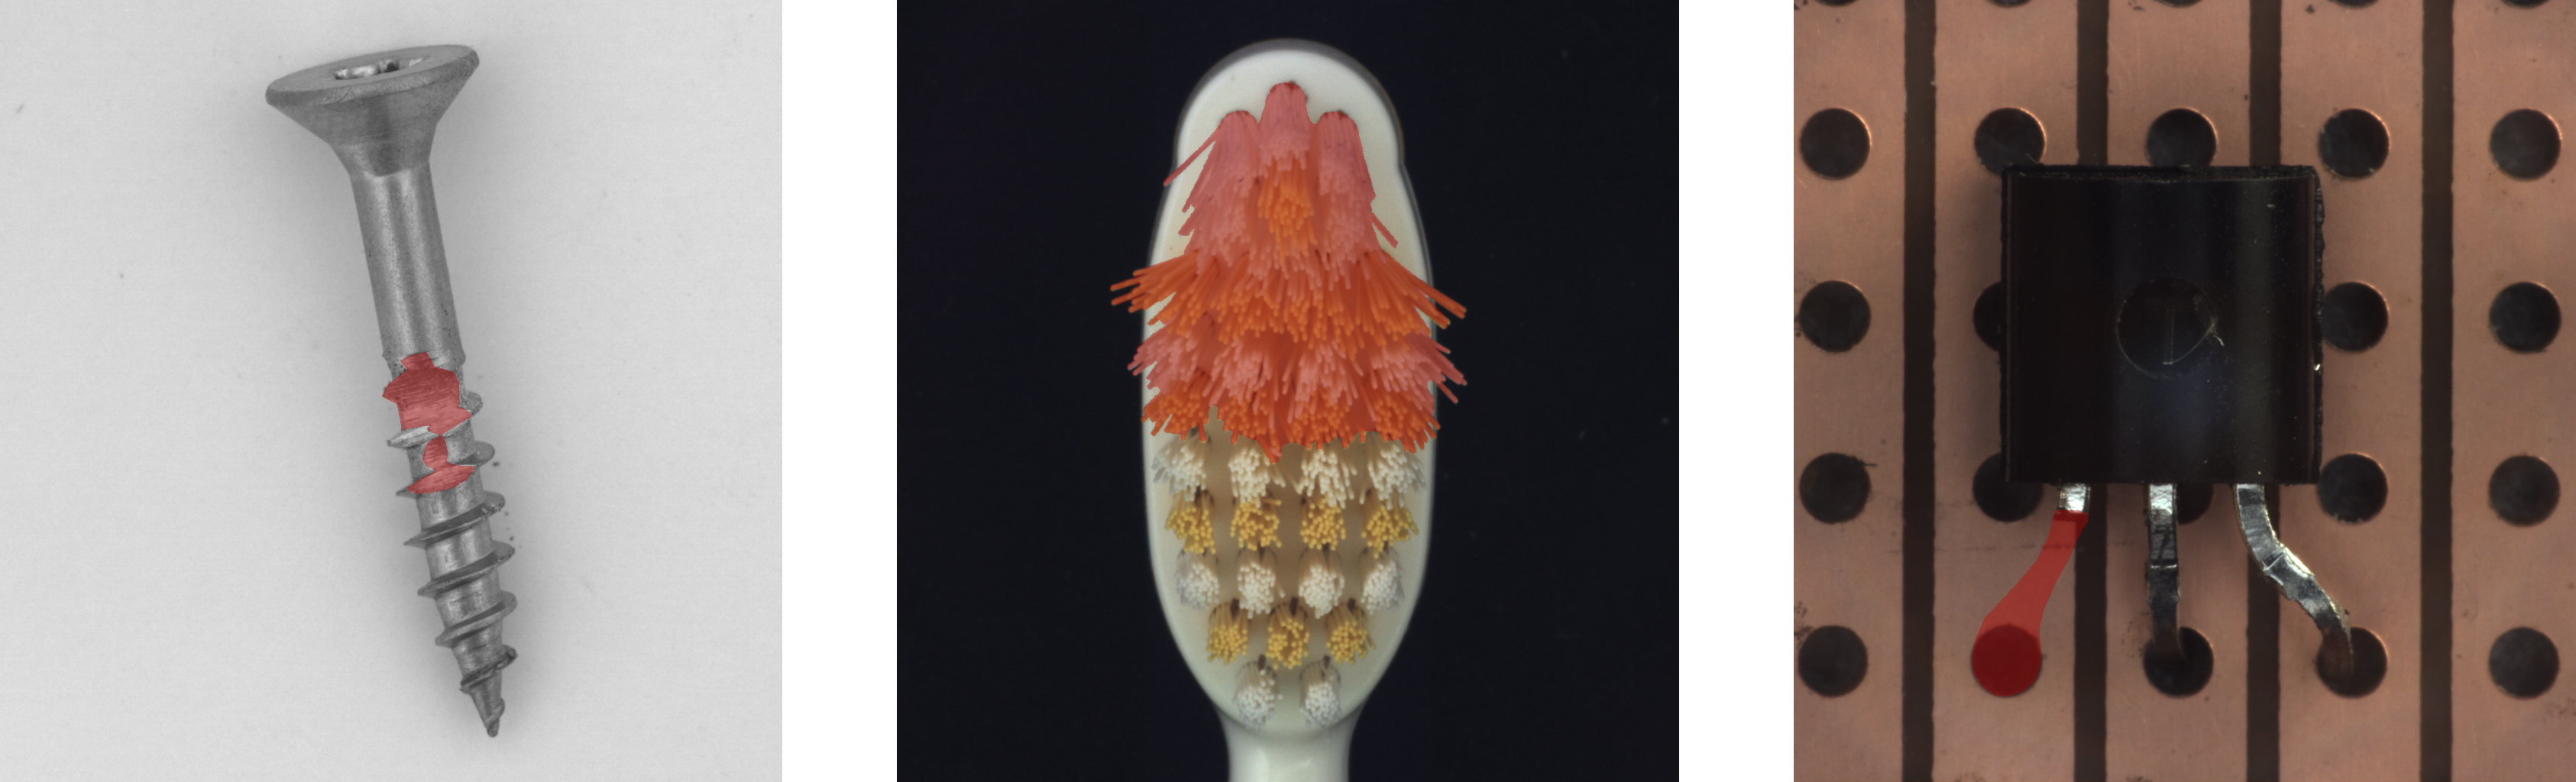
\includegraphics[width=\textwidth]{imgs/mvtec-example-objects.jpg}
\label{fig:methods:objects-example}
\end{figure}

\begin{figure}[h!]
\caption{An example of a piece of leather, tile and grid that are defective.}
\centering
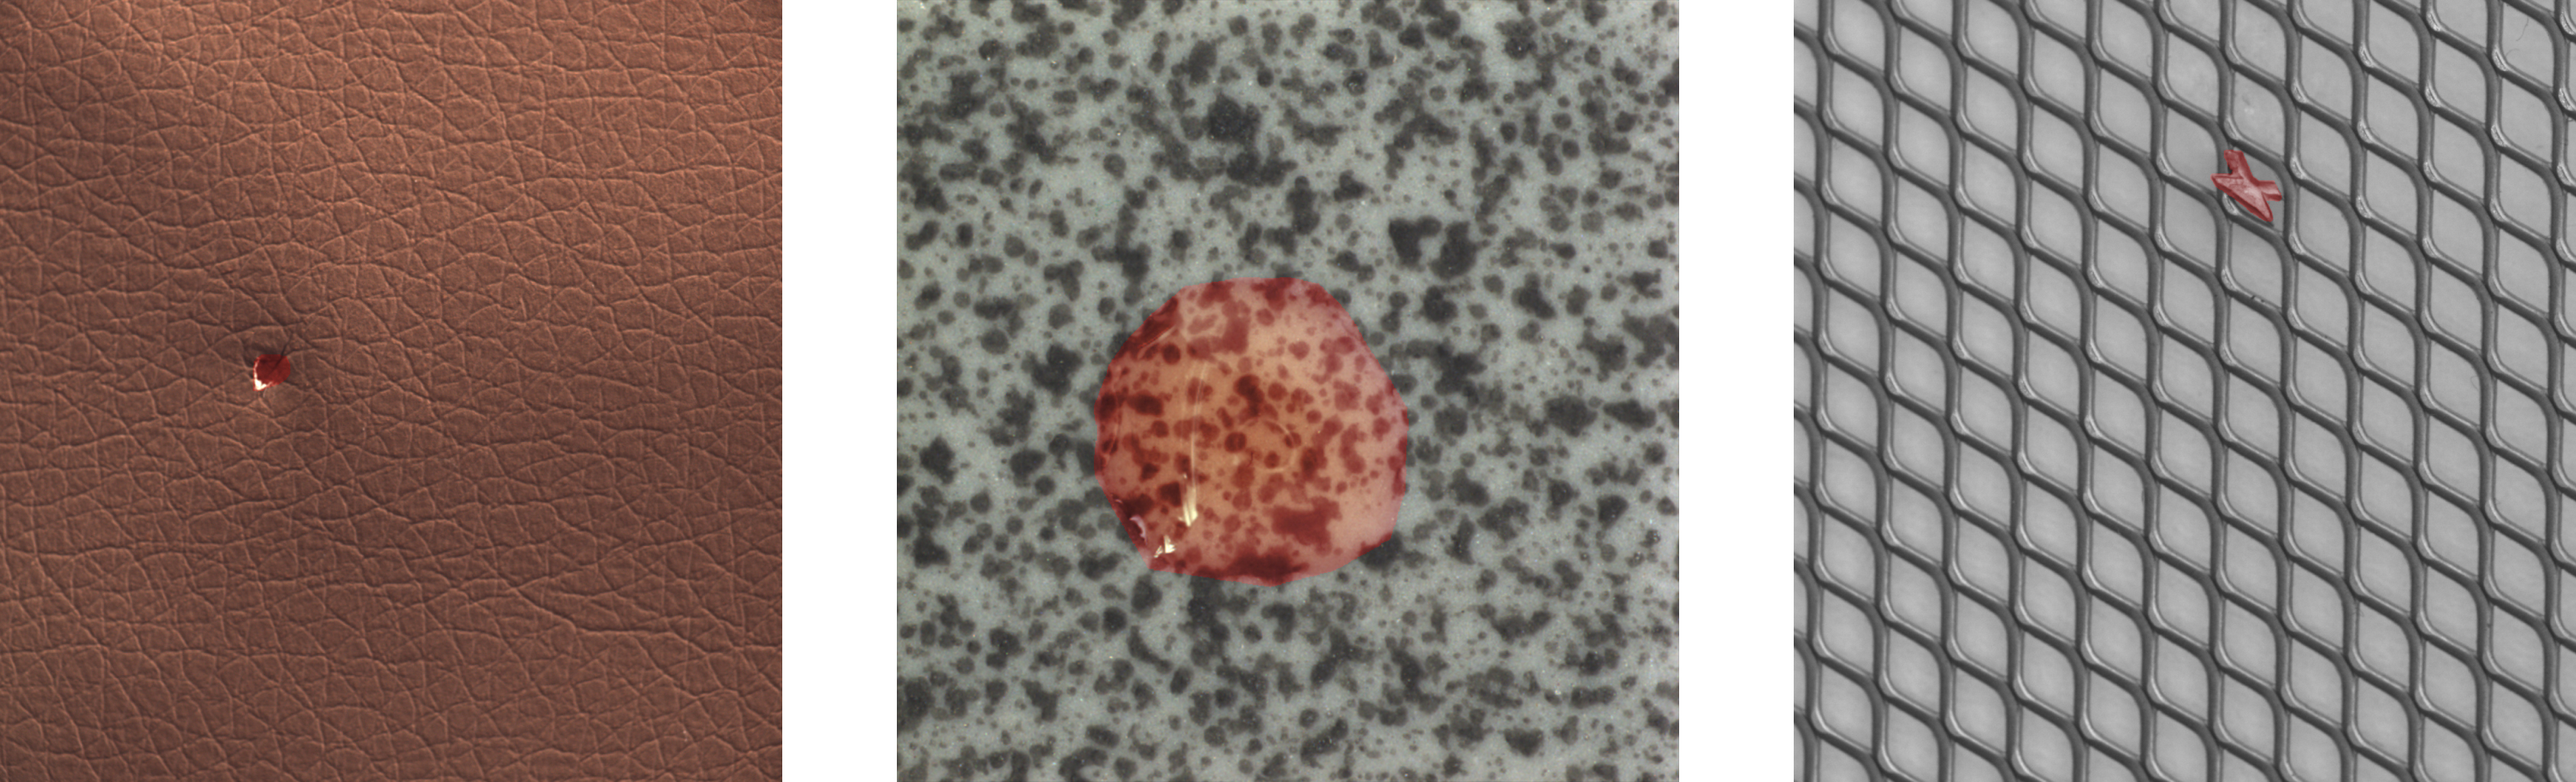
\includegraphics[width=\textwidth]{imgs/mvtec-example-textures.jpg}
\label{fig:methods:textures-example}
\end{figure}

In figure \ref{fig:methods:objects-example} we see three different object-type images with defects. Compared to figure \ref{fig:methods:textures-example} where we have examples of textures. These different types of images allow us to test our model to do both detailed texture synthesis and structure inpainting. In the case of anomaly detection the defects on the textured images are smaller and require finer reconstruction of the texture details when compared to the larger objects where the anomalies usually consist of larger deformations or missing elements.

\section{Experimental setup}

\subsection{Model structure}

\subsection{Training}

\subsection{Inference}

\subsection{Metrics}

\improvement{Need to think about order of subsections here}

To be able to quantify the performance of our models we require metrics that are suitable for the inpainting task that we are performing. This means that we need a loss function that takes into account that our dataset contains both textures and objects. For this we use a combination of structural similarity, gradient magnitude similarity and a pixel-wise L2 loss. Then to evaluate the performance we use the standard ROC AUC metric that is commonly used to evaluate models used for anomaly detection and was also used in the original inpainting paper \cite{pirnay_inpainting_2021, zavrtanik_reconstruction_2021}.


\subsubsection{Loss}

Since we try to recreate the model from \cite{pirnay_inpainting_2021} we also use a similar loss function. Which is equal to the one used in \cite{zavrtanik_reconstruction_2021}.

Our loss function L consists of three parts. The first part is a pixel-wise $L_2$ loss. This does not take into account perceptual differences, since it assumes that all pixels in the images are independent. Therefore we also use the structured similarity index (SSIM) \cite{bergmann_improving_2019} and the multi-scale gradient magnitude similarity (MSGMS) \cite{xue_gradient_2014, zhang_gradient_2017}.

The SSIM is a metric that looks at dependencies between regions of an images by including luminance, contrast and structural information. This means that it assumes that our model is able to find those structures. MSGMS is similar in that it looks at local image quality but does not focus on those structures.
\\
Before we determine the full loss function we first formulate these three base parts given our original patch $P$ and the reconstruction $\hat{P}$ for that patch.

\begin{align}
L_{SSIM} = \frac{1}{N_p} \sum_{x=1}^{W}\sum_{y=1}^{H}{} {1 - SSIM_{(x,y)}(P_l, \hat{P}_l)}
\end{align}

where $N_p$ is the number of pixels of the patch $P$. The $SSIM_(x,y)$ is the SSIM result for the two pixel in the patch and the reconstruction with $(x,y)$ being the center.

\begin{align}
L_{GMS} = \frac{1}{4} \sum_{l=1}^{4} \frac{1}{N_l} \sum_{x=1}^{W_l}\sum_{y=1}^{H_l}{} {1 - GMS_{(x,y)}(P_l, \hat{P}_l)}
\end{align}

where $N_l$ is the number of scales. $P_l$ and $\hat{P}_l$ the scaled version of the patches and $GMS_{(x,y)}(P_l, \hat{P}_l)$ gives the GMS map of those scaled patches at the pixel location $(x,y)$.

We can then define our complete loss function as 

\begin{align}
L(P, \hat{P}) = L_2(P, \hat{P}) + \alpha \; L_{GMS}(P, \hat{P}) + \beta \; L_{SSIM}(P, \hat{P})
\end{align}

with $\alpha$ and $\beta$ being loss weights for the individual components.

\subsubsection{Evaluation}

To be able to compare two different transformer models we will use the ROC AUC, which is standard for visual anomaly tasks \cite{pirnay_inpainting_2021, zavrtanik_reconstruction_2021, schlegl_unsupervised_2017, li_cutpaste_2021, tsai_autoencoder-based_2021, xie_semisupervised_2021, bergmann_mvtec_2019}.

For this we will use the anomaly map $anomap(x)$ we obtained from the images in section \ref{sec:methods-setup-ad}.

We want to evaluate both the anomaly detection on the image-level and the anomaly segmentation on the pixel-level. For the last task we can directly use the anomaly map. For the image-level detection we take the maximum pixel value from the anomaly map as a single anomaly score for the whole image.

\subsection{Anomaly detection}\label{sec:methods-setup-ad}



\section{Linear Inpainting Transformers}

Our linear inpainting transformers are almost identical to the transformer model used by Pirnay et al. \cite{pirnay_inpainting_2021}.



\subsection{Training}

\todo{1. Machines used 2. Early stopping 3. Train/test selection}

\subsection{Best result selection}

\todo{Lowest loss etc}

\subsection{}